% -*- TeX-engine: luatex; fill-column: 101; eval: (auto-fill-mode -1); eval: (visual-fill-column-mode 1); eval: (visual-line-mode 1); eval: (adaptive-wrap-prefix-mode 1) -*-
%% EDITOR: Cover sheet created separately
% \begin{titlepage}
% 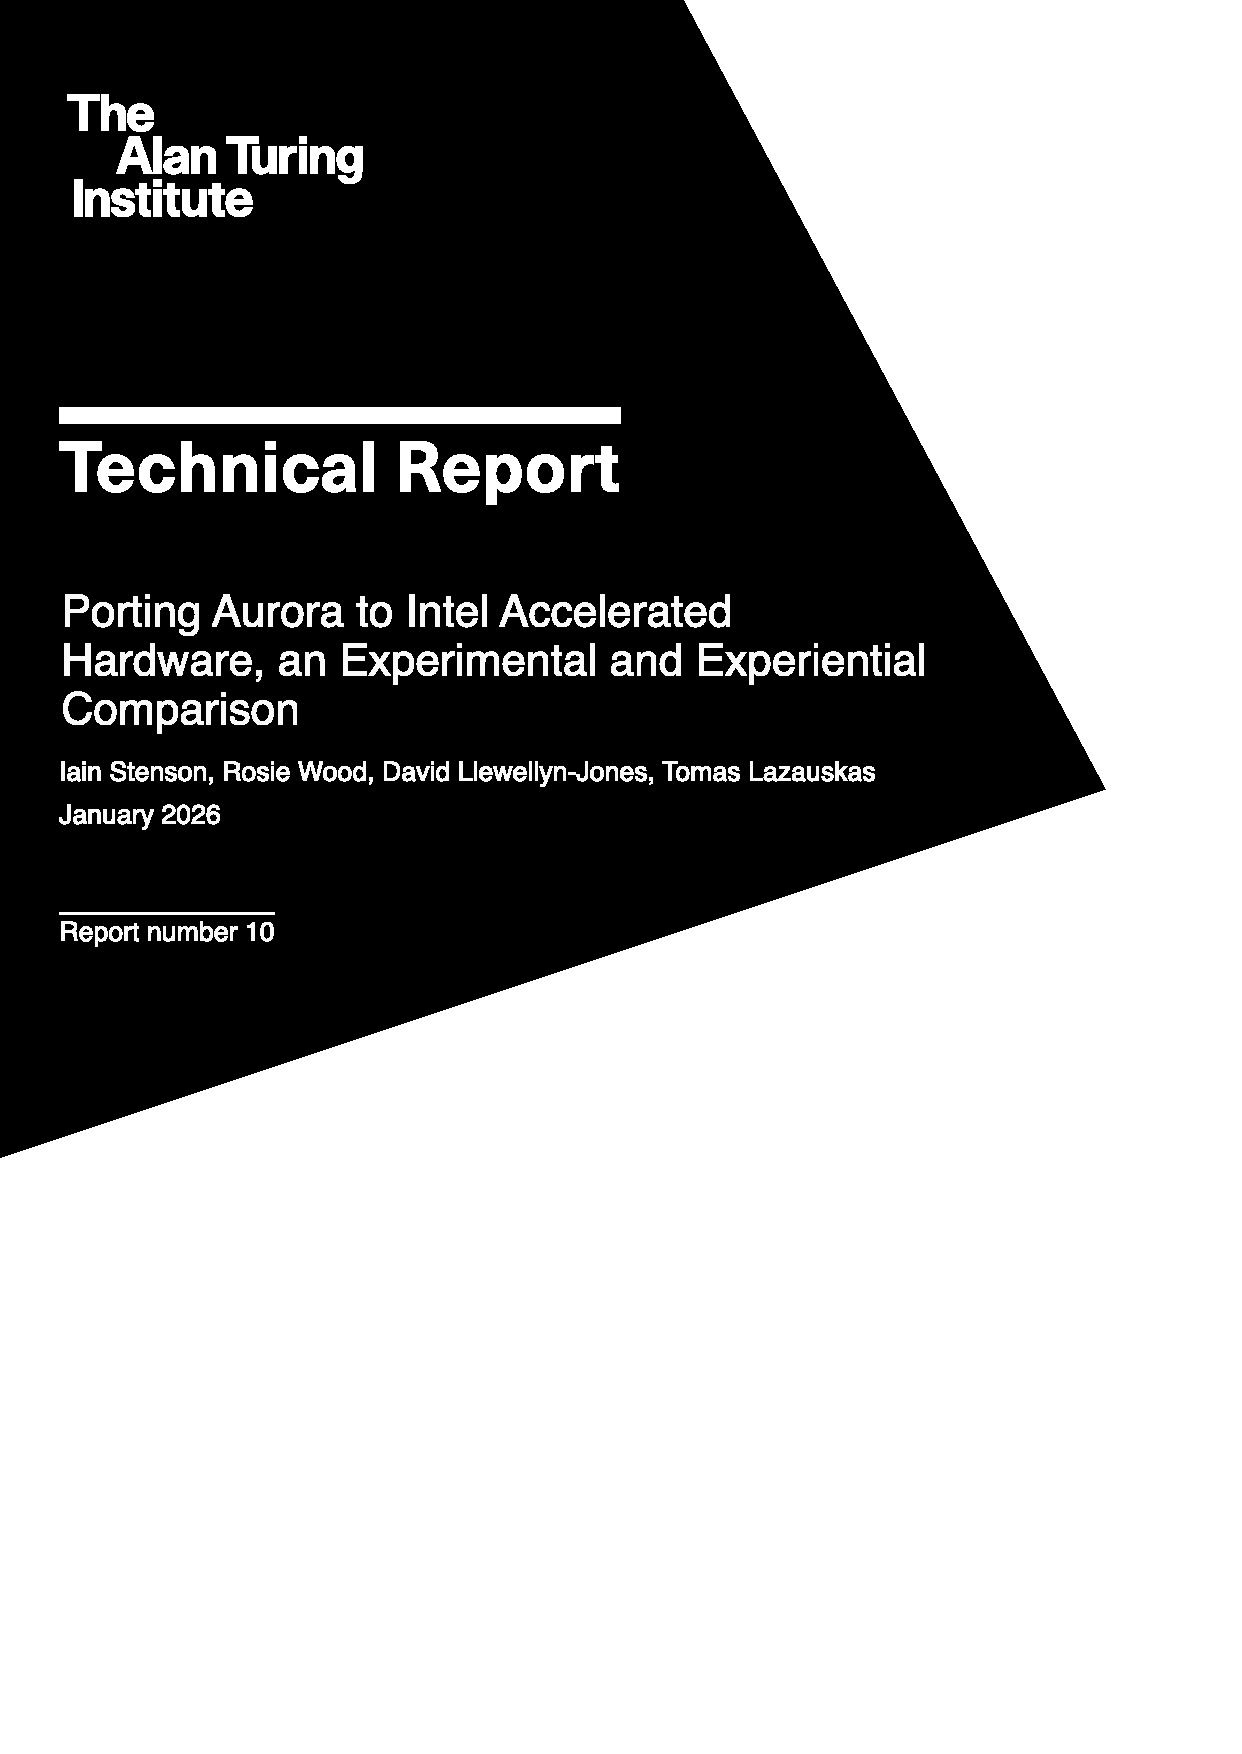
\includepdf{diagrams/tech-report-title-page}
% \end{titlepage}
% \title{Porting Aurora to Intel Accelerated Hardware, an Experimental and Experiential Comparison}
% \author{Iain Stenson, Rosie Wood, David Llewellyn-Jones, Tomas Lazauskas}
\begin{abstract}
    Dawn is an AI-optimised High Performance Computing system funded under the AI Research Resource programme in the UK. Unlike other similar systems it uses Intel\textsuperscript{\tiny\textregistered} Data Center GPU Max 1550 GPUs, which are incompatible with the \textit{de facto} standard NVIDIA CUDA and AMD ROCm accelerator frameworks.

    This work explores the process and challenges of porting code originally developed for NVIDIA hardware onto the Intel hardware on Dawn. We used the Microsoft Aurora weather model as a test case, benchmarking inference and training speeds and comparing against the NVIDIA A100 GPUs used on the Baskerville High Performance Computing system.

    We find that single-GPU inference performance is comparable between the two systems, but that multi-GPU training on Dawn is consistently around 3 times slower, largely due to the need to use a composite device hierarchy to access the full 128 GiB of GPU memory. We also identify non-determinism in Dawn's default configuration that requires explicit mitigation, as well as numerical differences between the platforms in single- and half-precision floating-point operations.
\end{abstract}

\newpage
\setcounter{tocdepth}{2}
%% EDITOR: Changed baselinestretch
% {
%\renewcommand{\baselinestretch}{0.75}\normalsize
\tableofcontents
%}
\newpage

\section{Introduction}

Dawn is one of two AI-optimised HPCs funded by the UK government as part of the AI Research Resource (AIRR) programme \cite{applencourt1014dawn,mcintosh2024isambard}. Hosted at the University of Cambridge, Dawn differs from most UK HPCs in that it uses Intel GPUs as opposed to NVIDIA GPUs. Dawn was first made available for pioneer (early access) projects in April 2024 with full access to the broader community starting in April 2025.

While several Turing projects had the benefit of trialling the service during the early access period, the new architecture means it is nevertheless a relatively unknown quantity for researchers both inside and outside the Turing.

AI workloads are typically highly parallelisable and therefore able to make effective use of GPU compute to accelerate both training and inference. Both within the High Performance Computing space and in other areas NVIDIA enjoys relative market dominance. This has led to a scarcity of the most powerful GPUs from NVIDIA, particular due to increases in AI-driven workloads \cite{yoffie2024nvidia}.

In this environment the opportunity to diversify -- being able to deploy workloads to multiple different systems using a diversity of GPU architectures -- becomes an attractive proposition.

Given this context and the fact that Dawn eschews NVIDIA in favour of Intel GPUs, we wanted to find out about the challenges involved in porting a real-world AI workload -- known to work with NVIDIA GPUs and of relevance to Turing researchers -- onto the Intel-based Dawn supercomputer.

This work therefore explores the ease of porting code originally developed for NVIDIA hardware onto the Intel hardware on Dawn. We use the Microsoft Aurora weather model \cite{bodnar_foundation_2025} as a test case, investigate the ease of running Aurora on Dawn, and benchmark inference and training speeds against NVIDIA A100 GPUs on Baskerville HPC.

Our results show near-consistent inference outputs between the two HPCs: performing a seven day (28 time-step) roll-out yielded similar but not identical results on Dawn and Baskerville, with the two-metre temperature RMSE between the two reaching \qty{0.09}{\kelvin}. Average inference times were also comparable at around 6.2 seconds per time-step for Dawn and 6.1 seconds per time-step on Baskerville. However, training speeds were consistently around 3 times slower on Dawn versus Baskerville. We attribute this to the need to use a \textit{composite} device hierarchy when running Aurora on Dawn, in which both GPU tiles are treated as one single device and which is needed to access the full 128 GiB of GPU memory. Running a smaller version of the Aurora model using the \textit{flat} device hierarchy gave us training speeds more in line with those seen for Baskerville using the same model configuration.

As noted the results obtained were similar but not identical. We therefore also explored the extent to which the two systems differ in their outputs. Although the differences are real, the RMSE for 27 rollout steps amounted to 0.0937 K.  For a sense of scale, we can look at numbers provided by Weatherbench 2 \cite{rasp2024weatherbench2benchmarkgeneration} on the performance of IFS ENS (Integrated Forecasting System Ensemble), a numerical weather prediction system operated by the European Centre for Medium-Range Weather Forecasts (ECMWF) \textit{vs.}\ their analysis (a best-guess of the Earth system state, which are also used as the forecast's initial conditions).

Our difference of \qty{0.0937}{\kelvin} is relatively small next to the error of the mean of the IFS ENS, which is reported by Weatherbench 2 to be \qty{1.699}{\kelvin}. We explored the discrepancies in more detail by considering errors introduced when performing more basic operations of matrix multiplication and addition. We found that discrepancies were introduced through the use of \fphalf\ and \fpdouble\ calculations, whereas \bfhalf\ calculations yielded identical results on both systems.

\section{Aims}

The main purpose of this work can be summarised by the following four aims.

\begin{enumerate}
\item Show that Aurora can be set up and run on Dawn.
\item Test out inference in order to assess Dawn's ability to produce correct results.
\item Test out fine-tuning in order to assess the speed and efficiency of training models on Dawn.
\item Compare results obtained on Dawn with the same code running on Baskerville.
\end{enumerate}

\section{Summary}

Each section is prefaced with a brief list summarising our conclusions from the results discussed. As a preview of this we combine these lists into the single list below, which summarises our findings from across the entire text.

\begin{enumerate}
    \item Dawn uses Intel\textsuperscript{\tiny\textregistered} Data Center GPU Max 1550 GPUs; Baskerville uses NVIDIA A100 GPUs.
    \item Performing inference roll-out for 7 days (28 time-steps) showed similar but not identical results between Dawn and Baskerville, with the two-meter temperature RMSE between the two reaching \qty{0.09}{\kelvin}.
    \item Baskerville gave consistent results but additional configuration was required to avoid small variations between runs on Dawn.
    \item For inference, average step time was 6.2 seconds and 6.7 seconds on Dawn, using \textit{flat} and \textit{composite} hierarchies, respectively, compared to 6.1 seconds on Baskerville.
    \item Using multi-node and multi-GPU training, Dawn consistently ran approximately three times slower than Baskerville.
    \item Slower Dawn performance can be partially attributed to the need to use \textit{composite} device hierarchy on Dawn with a two times performance hit. Model sharding would likely be one approach to mitigating this.
    \item The CPU to GPU/XPU bandwidth on Dawn is consistently higher
      than on Baskerville by a factor of up to~4.4.
    \item Filesystem performance depends on caching, with Baskerville having faster un-cached reads and Dawn having faster cached reads.
    \item Measuring floating point matrix operation errors showed better accuracy using \fpsingle\ on Baskerville, better accuracy using \fphalf\ on Dawn and identical results across the two systems for \bfhalf.
    \item We experienced some reliability issues due to data centre upgrades with Dawn.
    \item We received timely support from the Dawn team throughout.
\end{enumerate}

\section{Set up}

In this section we describe the hardware, software and configurations used for our experiments.

\subsection{Summary}

The main outcomes of this section will be to show the following:

\begin{enumerate}
    \item Dawn uses Intel\textsuperscript{\tiny\textregistered} Data Center GPU Max 1550 GPUs; Baskerville uses NVIDIA A100 GPUs.
\end{enumerate}

\subsection{Dawn hardware}

Dawn hardware is detailed on the \href{https://docs.hpc.cam.ac.uk/hpc/user-guide/pvc.html#hardware_}{Cambridge CSD3 pages}.

Briefly, there are 256 nodes, each with four Intel\textsuperscript{\tiny\textregistered} Data Center GPU Max 1550 GPUs. Each GPU consists of two tiles (a.k.a. {\it stacks}) that can be treated as two independent devices with 64 GiB RAM or as one device with 128 GiB RAM.

Each node has 2 $\times$ Intel\textsuperscript{\tiny\textregistered} Xeon\textsuperscript{\tiny\textregistered} Platinum 8468 CPUs, giving a total of 96 cores.

\subsubsection{Dawn device hierarchy}
\label{section:devicehierarchy}

The Intel\textsuperscript{\tiny\textregistered} Data Center Max 1550 GPUs used by Dawn are based on the Ponte Vecchio architecture. These differ from the NVIDIA A100 GPUs in Baskerville in that each GPU is composed of two compute units, referred to as {\it tiles} or {\it stacks} (to avoid confusion with terminology used elsewhere, we refer to them here as {\it stacks}).

Each stack is made up of eight TSMC N5 compute tiles and four Intel 7 memory tiles on an Intel 7 Foveros base die. Connected to each die are four HBM2E memory tiles and a TSMC N7 SerDes connectivity tile, connected using dense embedded interconnect bridges (EMIB). A further EMIB joins the two stacks together \cite{ponteveccio_2022}. See Figure \ref{fig:ponteveccio-stacks} for a high-level illustration of the arrangement.

\begin{figure}[t]
\centering
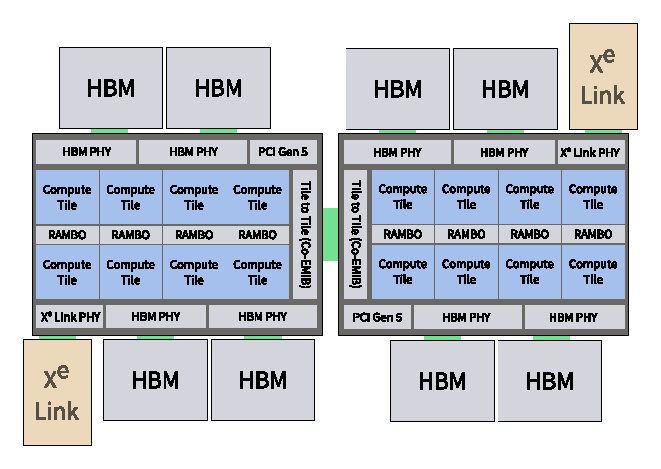
\includegraphics[width=0.8\linewidth]{diagrams/ponteveccio}
\caption{\label{fig:ponteveccio-stacks}Illustrative diagram showing the internal components of the Ponte Vecchio GPU architecture \cite{ponteveccio_2022}.}
\end{figure}

Intel\textsuperscript{\tiny\textregistered} Data Center Max 1550 GPUs can be used in two modes, called {\it hierarchies}. In the {\it flat\/} hierarchy, each stack is exposed as a separate GPU and addressable as if it were a different piece of hardware. In this mode there appear to be eight addressable GPUs on the node (2 stacks $\times$ 4 GPU cards). In the {\it composite} hierarchy, both stacks are treated as one root device composed of multiple sub-devices. Implicit scaling then means that the two stacks appear as a single GPU.

For our purposes the crucial difference between the two is that in {\it flat} mode we see two devices, each with 64 GiB of addressable High Bandwidth Memory, whereas in {\it composite\/} mode we see a single device with 128 GiB of addressable High Bandwidth Memory. The standard Aurora model requires approximately 80 GiB for training and hence its use is restricted to {\it composite} mode. We consider the performance impact of this restriction in Section \ref{section:modelsize}.

\subsubsection{Python environment}

On Dawn, we installed Aurora using a virtual environment with Python~3.11.9, microsoft-aurora v1.5.1, PyTorch 2.7.0 and \href{https://pytorch-extension.intel.com/installation?platform=gpu&version=v2.7.10%2Bxpu&os=linux%2Fwsl2&package=pip}{Intel Extension for PyTorch} v2.7.10+xpu (a.k.a. ``ipex'').
The ipex library is necessary because, until recently, PyTorch did not support Intel GPUs out of the box.
For single-GPU usage, only ipex is necessary. For multi-GPU work, the oneCCL Bindings for PyTorch library is also needed for collective communications. This is Intel's equivalent of \href{https://developer.nvidia.com/nccl}{NVIDIA's NCCL}.

Recent versions of PyTorch have introduced native support for Intel XPUs, including the XCCL distributed backend in \href{https://pytorch.org/blog/pytorch-2-8/}{PyTorch 2.8}. These changes were too recent to be used in this report, but our experience has been that the dependencies and setup required are greatly simplified with these newer versions of PyTorch.

\subsubsection{Modules}

As is common on HPC systems, Dawn uses environment modules to add or remove packages from the environment, applied using the \href{https://hpc-wiki.info/hpc/index.php?title=Modules&oldid=5007}{{\tt module} tool}. In order to use the oneCCL Python package, we needed to load some of the \href{https://www.intel.com/content/www/us/en/developer/tools/oneapi/base-toolkit.html#gs.mqrwie}{OneAPI Toolkit}, which is a collection of tools and libraries for working with Intel hardware.

We loaded the following modules:
\begin{enumerate}
    \item {\tt default-dawn}
    \item {\tt lua/5.3.6/gcc}
    \item {\tt intel-oneapi-mkl/2025.0.1}
    \item {\tt intel-oneapi-mpi/2021.14.1}
    \item {\tt intel-oneapi-ccl/2021.14.0}
\end{enumerate}

These include Intel's Math Kernel Library, the Intel implementation of MPI multiprocessing, and the Intel CCL libraries.

When we shared an early draft of this report with the Dawn team they noted that these modules were not the latest versions available. Concerned that this may have affected our results, we performed a subset of training runs to compare training times using the different modules. We found that there was no significant difference between the times for the training using the two different sets of modules. For details of this comparison, please see Appendix \ref{appendix:rhel}.

\subsubsection{Partition Information}

On Dawn, we used the pvc-9 partition. This used the Rocky Linux 9.6 (Blue Onyx) operating system and x86-64 architecture.

\subsection{Baskerville hardware}

Since one of the aims of this work is to compare the deployment of Aurora on Dawn with deployment on a more traditional CUDA-based system, we use the Baskerville Tier 2 High Performance Computer system as a comparison.

Baskerville hardware is detailed in the \href{https://docs.baskerville.ac.uk/system/}{Baskerville documentation}.

Baskerville offers NVIDIA A100 GPUs; we used the 80 GiB variants of these to ensure we had enough memory to perform fine-tuning of Aurora. Each node has four such GPUs and 2 $\times$ Intel\textsuperscript{\tiny\textregistered} Xeon\textsuperscript{\tiny\textregistered} Platinum 8360Y CPUs, giving a total of 72 cores at \qty{2.4}{\giga\hertz} (with boost to \qty{3.5}{\giga\hertz}) and 512 GiB RAM (16 $\times$ 32 GiB DDR4).

Baskerville GPUs offer a typical arrangement for running AI workflows, similar to the \href{https://learn.microsoft.com/en-us/azure/virtual-machines/sizes/gpu-accelerated/nca100v4-series}{NC\_A100\_v4 series} of virtual machines available on Azure.

\subsubsection{Python environment}

On Baskerville, we initially attempted to create a Python virtual environment matching that used on Dawn. However, when using Python 3.11, PyTorch 2.7.0 and microsoft-aurora 1.5.1, we found that running Aurora gave us an {\tt illegal memory access} error. This error has been reported multiple times on the Aurora repository and is thought to be due to dependency issues (see, for example, \href{https://github.com/microsoft/aurora/issues/121}{issue 121} and \href{https://github.com/microsoft/aurora/issues/125}{issue 125}). We were unable to resolve the error. Thus, on Baskerville, we installed Aurora using a virtual environment with Python 3.10.4, microsoft-aurora v1.5.2 and PyTorch v2.0.1+cu117. This allowed us to run the Aurora model without encountering the illegal memory access error. After discussion with the Dawn technical team, we decided that these version mismatches would not have a significant impact on our results. However, future work may involve looking into this illegal memory error further. One viable solution would be to use a containerised setup.

\subsubsection{Modules}

On Baskerville we loaded the following modules:
\begin{enumerate}
    \item {\tt baskerville}
    \item {\tt bask-app/live}
    \item {\tt PyTorch/2.0.1--foss-2022a-CUDA-11.7.0}
    \item {\tt torchvision/0.15.2-foss-2022a-CUDA-11.7.0}
\end{enumerate}

\subsection{ERA5 dataset}

We downloaded data from the \href{https://cds.climate.copernicus.eu/datasets/reanalysis-era5-single-levels?tab=overview}{ERA5} dataset as per the \href{https://microsoft.github.io/aurora/example_era5.html}{Aurora documentation}.

We downloaded 9 days' worth of data at 6 hour time-steps (36 time-steps total) from 2023-01-01 to 2023-01-09 and at times of 00:00, 06:00, 12:00 and 18:00. This dataset took up around 3.6 GiB (3.63 GiB) on disk as netCDF files. The variables provided are the following:

\begin{enumerate}
\item Static variables: {\tt z}, {\tt slt}, {\tt lsm}.
\item Surface variables: {\tt 2t}, {\tt 10u}, {\tt 10v}, {\tt msl}.
\item Atmospheric variables: {\tt t}, {\tt u}, {\tt v}, {\tt q}, {\tt z}.
\end{enumerate}
7
The map resolution is $1440 \times 721$ with 13 atmospheric levels.

\section{Inference}

We organised our experiments into several stages. First we deployed our model to the two High Performance Computing systems described in the previous sections and ensured that it ran correctly in both environments.

The first important element of this was to ensure that \textit{inference} was working correctly on both systems.

In this section we detail how we performed experiments to test inference and, in particular, whether the two systems produced different results. Where differences were apparent we look into more detail about the reasons for and characteristics of these differences.

\subsection{Summary}

In this section we will establish the following:

\begin{enumerate}
    \item Performing inference roll-out for 7 days (28 time-steps) showed similar but not identical results between Dawn and Baskerville, with RMSE between the two reaching \qty{0.09}{\kelvin}.
    \item Baskerville gave consistent results but additional configuration was required to avoid small variations between runs on Dawn.
    \item Inference timings were roughly comparable for Dawn and Baskerville with an average step time of 6.2 and 6.7 seconds on Dawn, using \textit{flat} versus \textit{composite} hierarchies, respectively, compared to 6.1 seconds on Baskerville.
\end{enumerate}

\subsection{Experimental setup}

We ran inference using the ERA5 dataset as per the \href{https://microsoft.github.io/aurora/usage.html}{Aurora documentation}.

We ran this for 28 steps (7 days), using the default 6 hour time-step, starting from the two data points at 2023-01-01 00:00 and 06:00. We used the Aurora checkpoint {\tt aurora-0.25-pretrained.ckpt} available from \href{https://huggingface.co/microsoft/aurora}{Hugging Face}. We repeated this 4 times on both Dawn and Baskerville and calculated an average of these for plotting.

On Dawn, we were able to run inference using both \textit{flat} and \textit{composite} device hierarchies.

\subsection{Results}
\label{section:results}

We compared our Dawn inference results with Baskerville and plotted the results. These can be seen in Figures \ref{fig:pvg-Dawn}--\ref{fig:errors}.

The left-hand plots of figures \ref{fig:pvg-Dawn} and \ref{fig:pvg-bask} show the predicted two-meter temperature after a 7 day rollout on Dawn and Baskerville, respectively. The right-hand sides of these figures show the ground truth values, taken from the ERA5 dataset.
From these, we can see both sets of predicted values look very similar, suggesting that both Dawn and Baskerville have generated very similar results.

We can quantify these results more accurately by calculating the Root Mean Square Error (RMSE) across the two systems and between the two systems. In Figure \ref{fig:errors} we perform a four-way comparison. The top row shows the error between the predicted values and ground truth for two-meter surface temperature after a 7 day rollout on Dawn (left) and Baskerville (right). The colour scale is between \qty{0}{\kelvin} and \qty{5}{\kelvin}. The bottom row shows the RMSE between the two sets of predicted values (Dawn and Baskerville) and the two sets of ground truth values.

We can see from the top row of Figure \ref{fig:errors} that both Dawn and Baskerville diverge from the ground truth values, and do so in similar global regions. The RMSE between predicted and ground truth results on Dawn is \qty{3.202056}{\kelvin}. We'd hope to therefore see a very similar error on Baskerville and, in fact, the RMSE there is \qty{3.203108}{\kelvin}.

\begin{figure}[t]
\centering
\includegraphics[width=1.0\linewidth]{plot-pvg-Dawn.pdf}
\caption{\label{fig:pvg-Dawn}Comparison of prediction {\it vs.}\ ground truth after 7 day rollout for the two-meter temperature in the range (\qty{223.15}{\kelvin}, \qty{323.15}{\kelvin}), generated on Dawn.}
\end{figure}

\begin{figure}[t]
\centering

\includegraphics[width=1.0\linewidth]{plot-pvg-bask.pdf}
\caption{\label{fig:pvg-bask}Comparison of prediction {\it vs.}\ ground truth after 7 day rollout for the two-meter temperature in the range (\qty{223.15}{\kelvin}, \qty{323.15}{\kelvin}), generated on Baskerville.}
\end{figure}

For this work the key comparison isn't between the predicted values and ground truth but rather between the two systems. From the bottom left plot, we see the RMSE between Dawn and Baskerville predictions is \qty{0.0936902}{\kelvin}, which gives an overall quantification of the impact that running on different systems and different configurations can have. Finally the RMSE between the ground truth results on Dawn and Baskerville is zero, which is to be expected since this is a subtraction between values loaded from the ERA5 data.

\begin{figure}[t]
\centering

\includegraphics[width=1.0\linewidth]{plot-errors.pdf}
\caption{\label{fig:errors}Absolute error comparison for two-meter temperature in K after 7 day rollout.}
\end{figure}

Figure \ref{fig:losses} compares the loss values from rollout across the two systems (see Section \ref{section:loss} for how the loss is calculated using the Mean Average Error equation). We see very similar results from both Dawn and Baskerville, with only very minor deviations occurring at later rollout steps.

\begin{figure}[t]
\centering

\includegraphics[width=1.0\linewidth]{plot-losses.pdf}
\caption{\label{fig:losses}Losses calculated using the Mean Average Error loss function (see Section \ref{section:loss}) for each rollout step comparing Dawn and Baskerville.}
\end{figure}

Figure \ref{fig:error-comparison} shows the RMSE and difference between Dawn and Baskerville predictions for two-meter temperature across the rollout. From the RMSE (left), we see a steady climb to \qty{0.09}{\kelvin} as the rollout progresses. From the difference (right), we see that, after a 7 day rollout, the predictions are distributed around 0, suggesting that there is no temperature bias between the Dawn and Baskerville results.

To try to understand the scale of discrepancy between the two systems, we compared the errors with the RMSE for the two-meter temperature values of the IFS ENS forecasts, as provided by Weatherbench 2. In Figure \ref{fig:error-weatherbench} we draw RMSE values for two example forecasts, plotting error bars to indicate the variability reflected by the errors we measured between the Dawn and Baskerville systems. We also draw the line for the Dawn and Baskerville RMSE values for comparison.

To take an explicit example, after 27 roll-out steps (162 hours) IFS ENS (mean) {\it vs.}\ Analysis RMSE as recorded by Weatherbench 2 was \qty{1.699}{\kelvin}. The equivalent for IFS ENS (1st member) {\it vs.}\ Analysis was \qty{2.554}{\kelvin}. The discrepancy between Dawn and Baskerville at this point was \qty{0.0937}{\kelvin}.

For these results we took the Weatherbench 2 data at the same resolution ($1440 \times 721$) as used for our results. However the times don't align: our data is for January 2023 whereas the Weatherbench 2 data is for 2022. These results are therefore not directly comparable, but we believe them to be broadly representative.

For the above results we have focused primarily on the two-meter temperature. Therefore Figure \ref{fig:varlosses} shows the loss for individual surface variables. Again, we see very similar results across the two systems.

\begin{figure}[t]
\centering
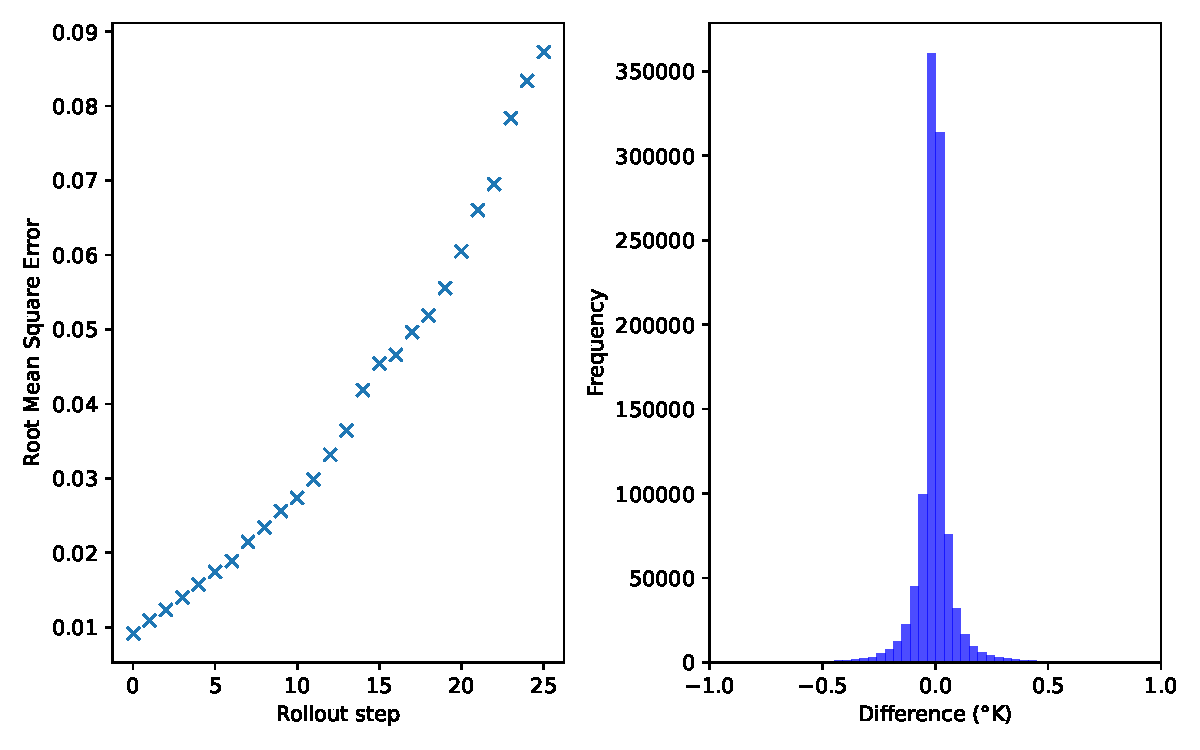
\includegraphics[width=1.0\linewidth]{diagrams/plot-error-line-and-histogram.pdf}
\caption{\label{fig:error-comparison} RMSE difference between Baskerville and Dawn two-meter temperature predictions after each rollout step. Distribution of Dawn predictions - Baskerville predictions after the final step. }
\end{figure}

\begin{figure}[t]
\centering
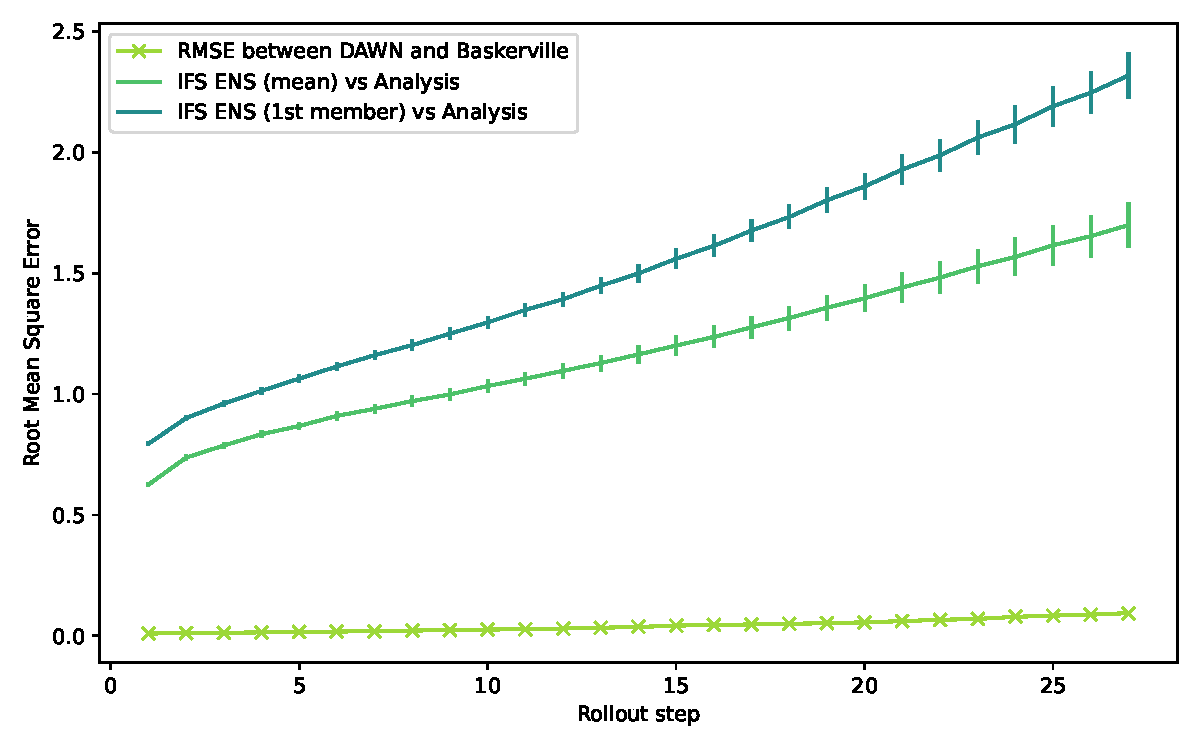
\includegraphics[width=1.0\linewidth]{diagrams/plot-weatherbench-comparison.pdf}
\caption{\label{fig:error-weatherbench} RMSE values generated by Weatherbench 2 for two high-performance forecasts compared to Analysis. Error bars show the ranges given differences between Dawn and Baskerville calculations. The RMSE between Dawn and Baskerville is also drawn for comparison.}
\end{figure}

\begin{figure}[t]
\centering

\includegraphics[width=1.0\linewidth]{plot-var-losses.pdf}
\caption{\label{fig:varlosses}Mean Absolute Error loss for individual variables for each rollout step comparing Dawn and Baskerville.}
\end{figure}

\subsubsection{Reproducibility between runs}
\label{section:reproducibility}

We ran four repeats on both Dawn and Baskerville to check reproducibility between runs. We calculated the standard deviation between runs and plotted these for two-meter surface temperature after a 7 day roll-out. Results are shown in Figure \ref{fig:std-dev-comparison}. We see there is variation when running repeats on Dawn, whereas Baskerville produces consistent results.

\begin{figure}[t]
\centering
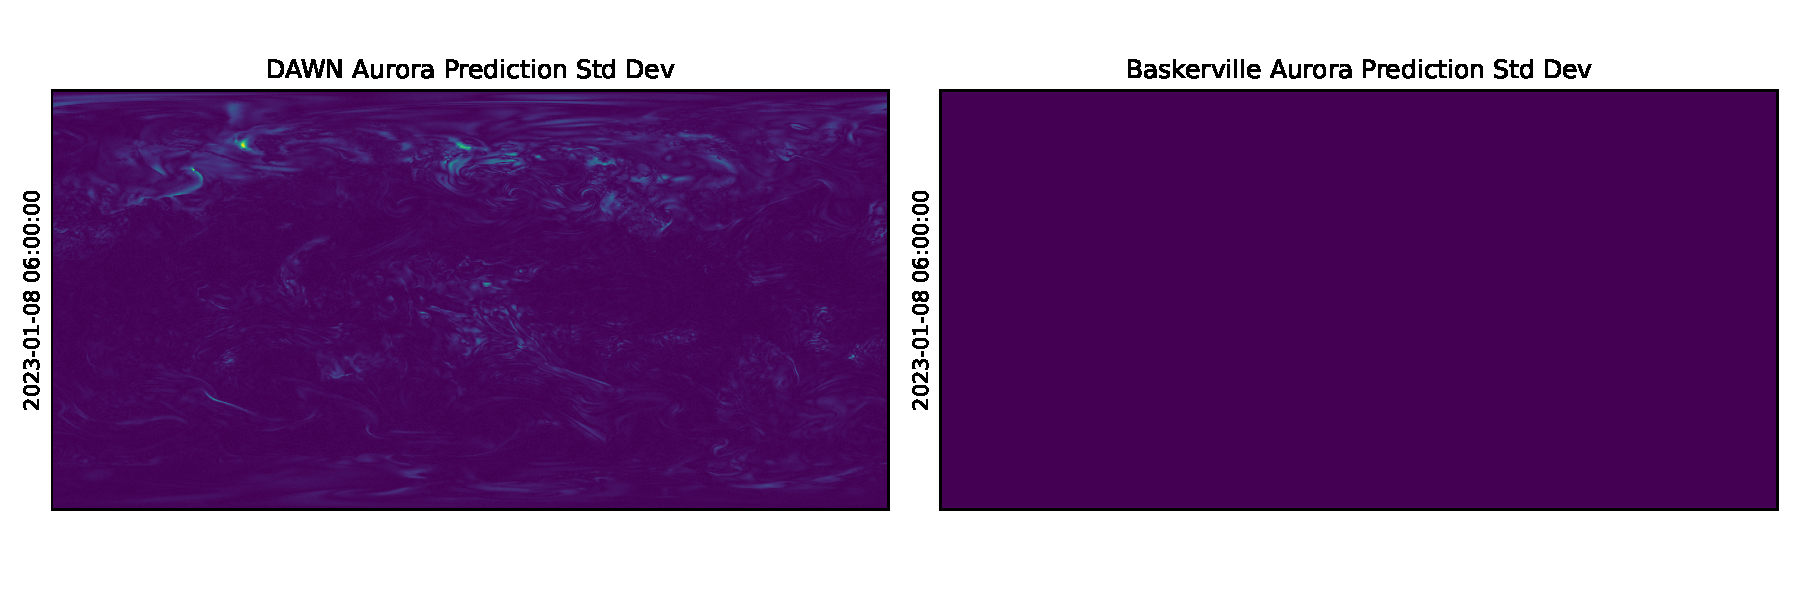
\includegraphics[width=1.0\linewidth]{diagrams/plot-std-dev-comparison.pdf}
\caption{\label{fig:std-dev-comparison} Standard deviation between 4 different repeats on Dawn (left) and Baskerville (right).}
\end{figure}

To avoid this and enforce consistent behaviour across runs on Dawn our code required additional configuration options to be added to the inference code preamble:

\begin{lstlisting}[language=Python]
torch.use_deterministic_algorithms(True)
torch.utils.deterministic.fill_uninitialized_memory = False
torch.xpu.random.manual_seed_all(42)
\end{lstlisting}

The first line enforces \textit{``algorithms which, given the same input, and when run on the same software and hardware, always produce the same output''}. When enabled, a {\tt RuntimeError} will be thrown if a required deterministic algorithm isn't available; however this didn't happen for our code.

Use of uninitialised memory can also cause nondeterministic behaviour in some cases. One solution for avoiding this is to fill all uninitialised memory before use, which can be configured by setting {\tt fill\_uninitialized\_memory} to {\tt True}. Since this impacts performance it is better to avoid this if it is not needed.

We tested with this option both set to {\tt True} and {\tt False} and established that this did not affect the results. We therefore disabled it for our runs to avoid the performance penalty.

Setting the random seed also required additional intervention. Typically we could call something like {\tt torch.manual\_seed(42)}, which is intended to set the seed across all devices. However we found it necessary to call the XPU-specific {\tt torch.xpu.random.manual\_seed\_all(42)} to ensure deterministic behaviour. This is important to be aware of, given it is an XPU-specific requirement.

\subsubsection{Time comparison}

For all inference timings, we exclude the time for the first time-step due to set-up overheads.

On Dawn, running inference using \textit{flat} device hierarchy gave an average time-step of 6.21 seconds. The total time for doing a rollout of 28 steps was 185.29 seconds and the total time for running the inference code, including loading data and the Aurora model, was 248.45 seconds. Running inference using \textit{composite} device hierarchy gave an average step time of 6.72 seconds. The total time for doing a rollout of 28 steps was 199.70 seconds and the total time for running the inference code was 262.76 seconds.

For comparison, running the same inference steps on Baskerville gave an average step time of 6.09 seconds. The total time for all 28 steps was 180.54 seconds. The total run time, including data and model loading, was 255.48 seconds. Given the small variation between runs, these results are broadly in line with those from Dawn, suggesting similar overall performance. Table \ref{tab:inference} summarises these results.

\begin{table}[t]
    \centering
 %   \hbadness=99999
    \begin{tabular}{@{}llrrrr@{}}
      \toprule
      System
      & Mode
      & \shortstack[r]{Mean\\ time-step ${}/\unit{\second}$}
      & \shortstack[r]{Time for\\ first step ${}/\unit{\second}$}
      & \shortstack[r]{Time for\\ 28 steps ${}/\unit{\second}$}
      & \shortstack[r]{Total\\ run time ${}/\unit{\second}$} \\ \midrule
        Dawn & \textit{flat} & 6.21&  17.56&185.29& 248.45\\
        Dawn & \textit{composite} & 6.72&  18.37&199.70& 262.76\\
        Baskerville & N/A& 6.09&  15.86&180.54& 255.48\\ \bottomrule
    \end{tabular}
    \caption{Inference timings.}
    \label{tab:inference}
\end{table}

\section{Fine-tuning}

Although it benefits from the GPUs on the two systems, inference is a relatively lightweight activity. Fine-tuning -- which involves further training the model taking a starting point using pre-established weights -- typically requires significantly more compute power than that needed for inference.

In order to fully compare the performance of this AI workload using the NVIDIA A100 GPUs of Baskerville and the Intel\textsuperscript{\tiny\textregistered} Data Center GPU Max 1550 GPUs of Dawn, we performed fine-tuning of the model on the two systems.

\subsection{Summary}

In the remainder of this section we will go on to show the following results.

\begin{enumerate}
    \item Using multi-node and multi-GPU training Dawn consistently ran approximately three times slower than Baskerville.
    \item Slower Dawn performance can be partially attributed to the need to use \textit{composite} device hierarchy on Dawn with a two times performance hit. Model sharding would likely be one approach to mitigating this.
    \item For the same training exercise, GPU energy usage on Dawn was substantially higher than on Baskerville.
\end{enumerate}

\subsection{Loss function}
\label{section:loss}

We defined our loss function (${\mathcal{L}}({\widehat{X}}^{t},{X}^{t})$) as per the Aurora paper \cite{bodnar_foundation_2025}:

\begin{align*}
{\mathcal{L}}({\widehat{X}}^{t},{X}^{t}) & = \frac{\gamma }{{V}_{{\rm{S}}}+{V}_{{\rm{A}}}}\left[\alpha \left(\mathop{\sum }\limits_{k=1}^{{V}_{{\rm{S}}}}\frac{{w}_{k}^{{\rm{S}}}}{H\times W}\mathop{\sum }\limits_{i=1}^{H}\mathop{\sum }\limits_{j=1}^{W}| {\widehat{S}}_{k,i,j}^{t}-{S}_{k,i,j}^{t}| \right)\right. \\
& \quad + \left.\beta \left(\mathop{\sum }\limits_{k=1}^{{V}_{{\rm{A}}}}\frac{1}{C\times H\times W}\mathop{\sum }\limits_{c=1}^{C}{w}_{k,c}^{{\rm{A}}}\mathop{\sum }\limits_{i=1}^{H}\mathop{\sum }\limits_{j=1}^{W}| {\widehat{A}}_{k,c,i,j}^{t}-{A}_{k,c,i,j}^{t}| \right)\right].
\end{align*}

Here $\gamma$ is a dataset-specific weight, ${V}_{{\rm{S}}}$ and ${V}_{{\rm{A}}}$ are the number of surface-level and atmospheric-level variables, respectively; $\alpha$ and $\beta$ are weights for the surface-level and atmospheric-level components of the loss, respectively; $H$ and $W$ are the number of latitude and longitude coordinates, respectively; $C$ is the number of atmospheric pressure levels; ${w}_{k}^{{\rm{S}}}$ is the weight associated with surface-level variable $k$ and finally ${w}_{k,c}^{{\rm{A}}}$ is the weight associated with atmospheric variable $k$ at pressure level $c$.

\subsection{Results}

We began by using the default device hierarchy (\textit{flat}) but found that this gave us an \texttt{Out of Memory error} due to the RAM limit of 64 GiB (half the full GPU), less than the required 80 GiB mentioned in the \href{https://microsoft.github.io/aurora/finetuning.html#computing-gradients}{Aurora documentation}. To resolve this we switched to \textit{composite} device hierarchy -- allowing both tiles to be treated as one single device -- and so were able to access the full 128 GiB RAM. This is done with the \texttt{ZE\_DEVICE\_HIERARCHY} environment variable. We were able to run fine-tuning in this set up.

We then moved on to test fine-tuning across multiple GPUs on the same node using distributed data parallel (DDP). Again, we used \textit{composite} device hierarchy so that each pair of tiles were treated as one single device with 128 GiB RAM. We found that using the PyTorch DDP class allowed us to distribute training, though, initially, we used duplicates of the same data on each worker.

We then created a \href{https://docs.pytorch.org/tutorials/beginner/basics/data_tutorial.html#creating-a-custom-dataset-for-your-files}{custom Dataset class} and used the PyTorch {\tt DistributedSampler} to take advantage of DDP by splitting our dataset across the different workers. Again, we set our device hierarchy to \textit{composite}. We found that we could run multi-GPU fine-tuning with this set up.

We proceeded to run fine-tuning on both Dawn and Baskerville using 34 time-steps (8.5 days). Since two time-steps are used as input, this equated to 32 iterations per epoch.

\subsubsection{Distributed Data Parallel (DDP)}
\label{section:time-comparison}

On Dawn and Baskerville, we ran multi-GPU fine-tuning with unsharded FSDP (equivalent to using DDP) using one node (one and four GPUs total), two nodes (two and eight GPUs total) and four nodes (four GPUs total). We did this using the PyTorch FSDP class and setting the FSDP sharding strategy to \texttt{NO\_SHARD}.

For these runs, we used a batch size of one ({\it i.e.,} one aurora \texttt{Batch}), the PyTorch {\tt DistributedSampler}, AdamW optimizer and our Aurora loss function for fine-tuning. To compare our different runs, we updated our model gradients only once per eight batches of data. This was to allow for the fact that when training with DDP and eight GPUs, eight batches of data would pass through our model (in eight parallel threads) before our model gradients would be updated. Thus, when running with one GPU, our model gradients should also only be updated after every eight batches of data. An iteration is therefore one forward pass (using an Aurora \texttt{Batch} with two time points to predict one future time point) and one backwards pass and, every eight iterations, we then do one optimiser step.

Timings for these runs are shown in tables \ref{tab:fine-tune-Dawn} and \ref{tab:fine-tune-bask}. Comparison of these two tables shows that Dawn is consistently running around 3 times more slowly than Baskerville.

\begin{table}[t]
    \centering
    \begin{tabular}{@{}llrrr@{}}
      \toprule
      Nodes
      & GPUs
      & \shortstack[r]{Compute time\\ per iteration ${}/\unit{\second}$}
      & \shortstack[r]{Wall-clock time\\ per iteration ${}/\unit{\second}$}
      & \shortstack[r]{Total\\ run time ${}/\unit{\second}$} \\ \midrule
        1 & 1 & 18.13& 18.13& 636.14\\
        1 & 4 & 17.76& 4.44& 212.96\\
        2 & 4 & 19.40& 4.85& 198.54\\
        4 & 4 & 19.60& 4.90& 201.28\\
        2 & 8 & 19.18& 2.43& 122.76\\ \bottomrule
    \end{tabular}
    \caption{Fine-tuning timings on Dawn.}
    \label{tab:fine-tune-Dawn}
\end{table}

\begin{table}[t]
    \centering
    \begin{tabular}{@{}llrrr@{}}
      \toprule
      Nodes
      & GPUs
      & \shortstack[r]{Compute time\\ per iteration ${}/\unit{\second}$}
      & \shortstack[r]{Wall-clock time\\ per iteration ${}/\unit{\second}$}
      & \shortstack[r]{Total\\ run time ${}/\unit{\second}$} \\ \midrule
        1 & 1 & 5.88& 5.88& 250.55\\
        1 & 4 & 6.83& 1.71& 120.34\\
        2 & 4 & 6.33& 1.58& 116.46\\
        4 & 4 & 6.22& 1.56& 117.84\\
        2 & 8 & 6.92& 0.87& 94.4\\ \bottomrule
    \end{tabular}
    \caption{Fine-tuning timings on Baskerville.}
    \label{tab:fine-tune-bask}
\end{table}

As the number of GPUs increases, there is an increase in the compute time per iteration due to the additional overhead in moving data between nodes and GPUs. However, this is more than offset by the additional parallelism. Consequently, although we don't see linear scaling in the total run time, it is not far off and in practice this matches our expectations for both systems. Assuming cost is proportional to GPU hours, the ``Compute time per iteration'' below can be seen as a proxy for the cost of running the training. More GPUs, therefore, means relatively more cost. However, more GPUs also sees the real time per iteration decreasing, which can be seen as a proxy for the wall-clock time needed to complete the training. Unsurprisingly there is a cost-time trade-off.

As an aside, comparing the results for ``Wall-clock time per iteration'', we note that on Baskerville increasing distribution across nodes turns out to be more performant than increasing distribution across GPUs on the same node. The opposite is true on Dawn.

\subsubsection{Resource utilisation}

We collected metrics for the training runs using two nodes with four GPUs on each.

In this case Baskerville streaming multiprocessor utilisation captured using {\tt nvidia-smi}\ consistently hit \qty{100}{\percent}. Memory utilisation fluctuated but reached at least \qty{76}{\percent} on the 80 GiB GPUs of Baskerville ({\it i.e.,} 61 GiB per GPU).

In comparison memory utilisation on Dawn consistently reached above \qty{60}{\percent} with a maximum of \qty{66.82}{\percent} ({\it i.e.,} 85.5 GiB per GPU). Due to access restrictions we were not able to capture processor utilisation on Dawn. Instead, we use GPU power consumption captured using {\tt xpu-smi}\ as a proxy for this. We explore energy usage in the next section.

\subsubsection{Energy usage comparison}
\label{section:energy-comparison}

For the same training exercise as in tables \ref{tab:fine-tune-Dawn} and \ref{tab:fine-tune-bask}, we captured GPU energy usage from {\tt xpu-smi}\ on Dawn and {\tt nvidia-smi}\ on Baskerville. We ran four repeats of the training and calculated the average energy used per training run by dividing by four. These energy readings include overheads such as model and data loading, process initialisation, as well as the energy to train the model. This choice was made to reflect the true energy requirements for running this entire workload. Tables \ref{tab:energy-bask} and \ref{tab:energy-dawn} show the average GPU energy per training run and average power draw per GPU for each configuration, with the Dawn-to-Baskerville energy ratio included alongside the Dawn results. These figures report GPU energy only and do not include CPU, memory, networking or system-level overheads.

Overall Dawn consumed between 3.3 times and 17.7 times more GPU energy than Baskerville for the same training exercise. This is driven by both higher mean power draw (between 1.9 and 3.9 times higher) and, in most configurations, longer elapsed time (between 0.85 and 3.26 times longer).

In terms of GPU energy usage, the lowest-energy configuration is one node with one GPU total on Baskerville (\qty{55267.94}{\joule}) and one node with one GPU total on Dawn (\qty{332511.66}{\joule}). The highest total energy occurs at two nodes with eight GPUs total on Baskerville (\qty{181773.66}{\joule}) and four nodes with four GPUs total on Dawn (\qty{1355921.92}{\joule}).

For average power draw per GPU, the lowest values are at two nodes with eight GPUs total on Baskerville (\qty{84.55}{\watt}) and four nodes with four GPUs total on Dawn (\qty{287.52}{\watt}), while the highest values occur at one node with one GPU total on both systems (\qty{209.15}{\watt} on Baskerville; \qty{386.30}{\watt} on Dawn).

\begin{table}[t]
    \centering
    \hbadness=99999
    \begin{tabular}{@{}llrr@{}}
      \toprule
      Nodes
      & GPUs
      & \shortstack[r]{Avg energy used\\ per training run ${}/\unit{\joule}$}
      & \shortstack[r]{Avg power draw\\ per GPU ${}/\unit{\watt}$} \\ \midrule
        1 & 1 & 55\,267.94 & 209.15 \\
        1 & 4 & 118\,982.26 & 98.17 \\
        2 & 4 & 86\,393.69 & 120.83 \\
        4 & 4 & 76\,523.08 & 138.63 \\
        2 & 8 & 181\,773.66 & 84.55 \\ \bottomrule
    \end{tabular}
    \caption{GPU energy usage for the same training exercise on Baskerville.}
    \label{tab:energy-bask}
\end{table}

\begin{table}[t]
    \centering
 \begin{tabular}{@{}llrrr@{}}
      \toprule
      Nodes
      & GPUs
      & \shortstack[r]{Avg energy used\\ per training run ${}/\unit{\joule}$}
      & \shortstack[r]{Avg power draw\\ per GPU ${}/\unit{\watt}$}
      & Energy ratio \\ \midrule
        1 & 1 & 332\,511.66 & 386.30 & 6.02 \\
        1 & 4 & 473\,221.48 & 364.58 & 3.98 \\
        2 & 4 & 761\,781.29 & 319.00 & 8.82 \\
        4 & 4 & 1\,355\,921.92 & 287.52 & 17.72 \\
        2 & 8 & 598\,843.44 & 327.95 & 3.29 \\ \bottomrule
    \end{tabular}
    \caption{GPU energy usage for the same training exercise on Dawn. Energy ratio is Dawn energy divided by Baskerville energy.}
    \label{tab:energy-dawn}
\end{table}

Overall, Dawn draws more power per GPU across every configuration and accumulates substantially more total energy, even when comparing like-for-like GPU counts.

\subsubsection{Effect of model size on training time}
\label{section:modelsize}

As mentioned previously, training thus far on Dawn has been done using \textit{composite} device hierarchy, meaning each GPU is exposed as a single root device (see Section \ref{section:devicehierarchy}). Doing so was necessary for the standard-size Aurora model to fit onto the GPU (particularly the memory-intensive backwards step).

To find out whether this device hierarchy had any performance penalty, we measured the time spent in the call to \texttt{loss.backward()} for models of different sizes.

To do this, we created a range of smaller Aurora models by varying encoder and decoder depths using the \texttt{encoder\_depths} and \texttt{decoder\_depths} arguments, respectively. In each case, we also reduced the number embedding dimension to 256, the numbers of heads in encoder and decoder layers to (4, 8, 16) and (16, 8, 4), respectively, and number of heads in aggregation and de-aggregation blocks to 8. All other parameters were kept as default. We ran this code on 1 node using 1 GPU.

Using encoder and decoder depths of $(x, x, x)$, an $x$ of 3 gives a model of roughly the same size as \texttt{AuroraSmall} (approx 300 MiB) and a value of 33 gives a model of roughly the same size as the standard Aurora (approx.\ 3 GiB). \textit{Flat} hierarchy ran out of memory for $x$ values of 14 and above.

\begin{figure}[t]
    \centering
    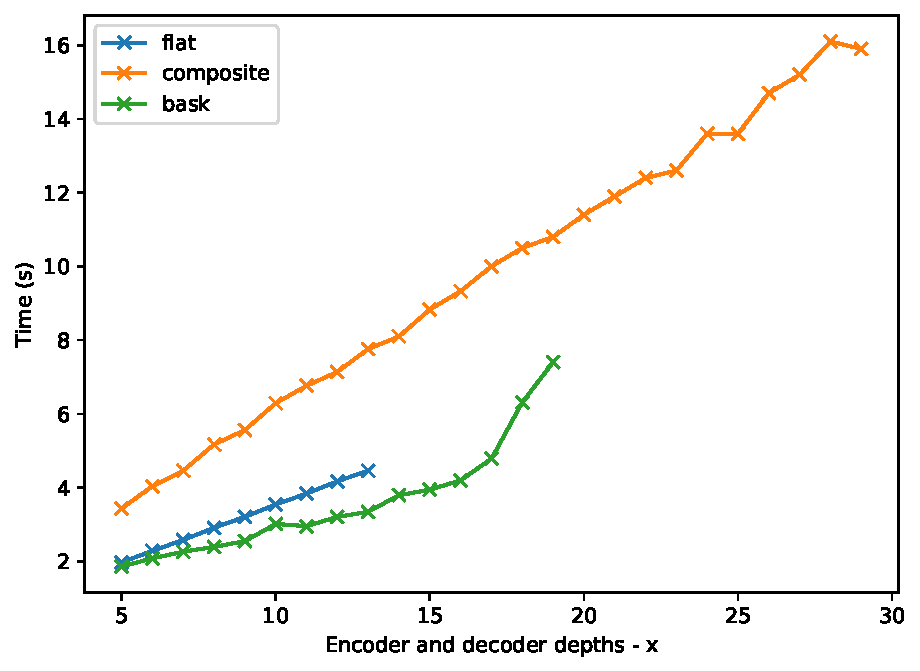
\includegraphics[width=0.9\linewidth]{diagrams/flat-vs-composite.pdf}
    \caption{Backprop Time \textit{vs.}\ Model Size}
    \label{fig:backprop-timings}
\end{figure}

As can be seen in Figure \ref{fig:backprop-timings}, training speeds when using \textit{flat} hierarchy were close to those of Baskerville, but were consistently slower when using \textit{composite} device hierarchy.

To investigate the difference between using \textit{flat} and \textit{composite} device hierarchies when training the Aurora model, we repeated the training experiments discussed in Section \ref{section:time-comparison} using a smaller Aurora model. We used the parameters defined above and set $x$=12 to give encoder and decoder depths of $(12, 12, 12)$.

We ran single-GPU fine-tuning with unsharded FSDP using 1, 2 and 4 GPUs. As before, we used a batch size of 1, the PyTorch {\tt DistributedSampler}, AdamW optimizer and our Aurora loss function for fine-tuning. For these runs we did not adjust the batch size dependent upon the number of parallel processes, and so updated our gradients after every iteration.

Results are shown in Table \ref{tab:flat-vs-composite-Dawn}. Note these are not directly comparable to the timings shown in Figure \ref{fig:backprop-timings}, which only relate to back propagation. From the table we can see that training using one tile and \textit{flat} hierarchy is up to twice as fast as using one full GPU with \textit{composite} device hierarchy. Likewise, using two tiles and \textit{flat} hierarchy is approximately twice as fast as using two full GPUs with \textit{composite} device hierarchy. This supports the results seen in Figure \ref{fig:backprop-timings}, which suggest that \textit{flat} device hierarchy results in double the training speed versus \textit{composite} hierarchy. Comparing Dawn training speeds against those from Baskerville, we can see that when using \textit{composite} device hierarchy, training runs approximately 3 times slower than Baskerville and when using \textit{flat} device hierarchy, training on Dawn runs approximately 2 times slower than Baskerville when using the same number of devices.

It is also worth noting that running on the 80 GiB A100 nodes on Baskerville, models of size $(20, 20, 20)$ or larger triggered out-of-memory errors. These models are technically smaller than the standard Aurora model but not directly comparable given the different structure resulting from changes to other parameters. The 128 GiB of memory available on the Intel GPUs in \textit{composite} mode allowed larger model sizes to be supported without sharding.

\begin{table}[t]
    \centering
    \begin{tabular}{@{}lllrrr@{}}
      \toprule
      GPUs
      & Devices
      & Hierarchy
      & \shortstack[r]{Compute time\\ per iteration ${}/\unit{\second}$}
      & \shortstack[r]{Wall-clock time\\ per iteration ${}/\unit{\second}$}
      & \shortstack[r]{Total\\ run time ${}/\unit{\second}$} \\ \midrule
          1  & 1&\textit{flat}& 6.86& 6.86& 257.43\\
  1& 2& \textit{flat}& 7.84& 3.92&176.54\\
          4& 4&\textit{flat}& 8.13& 2.03& 122.72\\
          4  & 8&\textit{flat}& 7.73& 0.97& 90.99\\
          1& 1&\textit{composite}& 11.10& 11.10& 391.70\\
  2& 2& \textit{composite}& 11.45& 5.72&259.46\\
          4& 4&\textit{composite}& 11.54& 2.89& 152.56\\
  1& 1& N/A (Bask)& 3.20& 3.20&145.53\\
  2& 2& N/A (Bask)& 3.25& 1.62&104.85\\
  4& 4& N/A (Bask)&  3.29& 0.82&81.72\\ \bottomrule
    \end{tabular}
    \caption{Comparison of fine-tuning timings on Dawn using 1 node and \textit{flat vs. composite} hierarchies and Baskerville.}
    \label{tab:flat-vs-composite-Dawn}
\end{table}

As a sanity check, and to isolate the data loader timings from the computation, we separately did a fine-tuning run with AuroraSmall. In it, we placed synchronisation calls before and after the backwards pass. On Baskerville 40 GiB A100 nodes, the backwards pass took around 0.7 seconds. On Dawn, with a \textit{flat} device hierarchy, the call to backwards took around 1.4 seconds. On Dawn, with \textit{composite} device hierarchy, the call to backwards took between 3 and 5 seconds.
This suggests that the low-level tensor algorithms, the GPU hardware or both could be responsible for the performance difference between Dawn and Baskerville.

Further work might involve techniques to reduce the maximum memory use, so that we can use a \textit{flat} device hierarchy without running out of memory.
More information on multi-stack architectures can be found in the Intel oneAPI online docs \cite{oneapi_multi_stack}.

\subsubsection{Fully Sharded Data Parallel (FSDP)}

With the \texttt{FULL\_SHARD} strategy, we have been able to reduce maximum GPU memory utilisation from approximately \qty{66}{\percent} to \qty{55}{\percent}. This uses a \texttt{ModuleWrapPolicy} to shard the encoder/decoder layers.

Attempts to shard more layer types have been found to give errors such as ``Inconsistent compute device and \texttt{device\_id} on rank 1: xpu:0 vs xpu:1''.  Attempts to use FSDPv2's \texttt{fully\_shard} wrapper function have resulted in \texttt{UR\_RESULT\_ERROR\_OUT\_OF\_RESOURCES} errors. Therefore, some further work is needed to understand how much more optimisation can be found with model and optimiser sharding.

For consistency, unless stated otherwise, all measurements in this document have been done with the \texttt{NO\_SHARD} strategy.

\section{Data transfer}

Given the results shown in the previous sections we were naturally keen to understand which parts of the computation were causing the difference.

To try to understand this better, we therefore ran several experiments to compare data transfer -- from disk to CPU and also from CPU to GPU -- on the two systems.

In this section we detail our experiments and present the results established.

\subsection{Summary}

In the remainder of this section we will go on to show the following results.

\begin{enumerate}
\item The CPU to GPU/XPU bandwidth on Dawn is consistently higher than on Baskerville by a factor of up to 4.4 times.
\item The filesystem performance depends on caching, with Baskerville having faster un-cached reads and Dawn having faster cached reads.
\end{enumerate}

\subsection{Results}
\label{section:transfer-results}

When training on large (\textgreater RAM) datasets, the bottleneck can sometimes be the rate at which data can be moved from disk to the compute device.

To compare platforms, we generated random tensors and pushed them to the GPU, with synchronisation calls immediately before and after.

\begin{table}[t]
    \centering
    \begin{tabular}{@{}rrr@{}} \toprule
      \shortstack[r]{Tensor Size\\ (MiB)}
      & \shortstack[r]{Dawn Bandwidth\\ (MiB/s)}
      & \shortstack[r]{Bask Bandwidth\\ (MiB/s)} \\ \midrule
          1 & 6\,162 & 3\,939 \\
  128 & 43\,620 & 9\,846\\
          1024 & 46\,876 & 10\,645\\ \bottomrule
    \end{tabular}
    \caption{Comparison of CPU to GPU/XPU bandwidth.}
    \label{tab:xpu-gpu-bandwidth}
\end{table}

Using the \texttt{dd} command to read ERA5 files gives us some sense of the file-system speed.

\begin{table}[t]
    \centering
    \begin{tabular}{@{}rrrr@{}} \toprule
        \shortstack[r]{File Size\\ (MiB)} 
      & \shortstack[r]{Cached\\ (Y/N)} 
      & \shortstack[r]{Dawn Bandwidth\\ (GiB/s)}
      & \shortstack[r]{Bask Bandwidth\\ (GiB/s)} \\ \midrule
           423 & N & 0.5 & 1.7 \\
   423 & Y & 7 & 5.5 \\ \bottomrule
    \end{tabular}
    \caption{Comparison of file-system bandwidth.}
    \label{tab:file-system-bandwidth}
\end{table}

\subsubsection{Data transfer with ERA5 data}

Using an ERA5 dataset containing 7 days' worth of data, we tested the time it took to load data first to RAM and then to GPU/XPU.

On Dawn, with device hierarchy set to \textit{composite}, we found that loading this dataset from disk (Lustre) to RAM took 25.6 seconds, roughly equivalent to $\qty{3.4}{\gibi\byte} / \qty{25.6}{\second} = \qty{0.13}{\gibi\byte\per\second}$. The average time to move each batch of training data from RAM to XPU was 0.0002 seconds, giving a total time of 0.0002 $\times$ 28 = 0.0056 s for all batches. This is roughly equivalent to $\qty{3.4}{\gibi\byte} / \qty{0.0056}{\second}
= \qty{607}{\gibi\byte\per\second}$ (assuming the full dataset is used during training).

On Baskerville, we found that loading this dataset from disk to RAM took 37.3 seconds, roughly equivalent to $\qty{3.4}{\gibi\byte} / \qty{37.3}{\second} = \qty{0.09}{\gibi\byte\per\second}$. The average time to move each batch of training data from RAM to GPU was 0.082 s, giving a total time of 0.082 $\times$ 28 = 2.296 s for all batches. This is roughly equivalent to $\qty{3.4}{\gibi\byte} / \qty{2.296}{\second} = \qty{1.48}{\gibi\byte\per\second}$ (assuming the full dataset is used during training).

These timings suggest data transfer both from disk to RAM and from RAM to GPU/XPU are faster on Dawn, in agreement with the results above. Notably, however, RAM to XPU transfer times seem to be approximately 410 times quicker on Dawn versus Baskerville. This may suggest an error in our code or calculation of RAM to XPU transfer time as this seems exceedingly fast.

\section{Calculation accuracy}
\label{section:errors}

Given that we experienced differences in results depending on the system, we wanted to establish whether this difference was present even at the level of basic mathematical matrix operations (addition and multiplication).

In this section we will describe the experiments we performed and the results collected for this.

\subsection{Summary}

In the remainder of this section we will go on to show the following result.

\begin{enumerate}
    \item Measuring floating point matrix operation errors showed better accuracy using \fpsingle\ on Baskerville, better accuracy using \fphalf\ on Dawn and identical results across the two systems for \bfhalf.
\end{enumerate}

\subsection{Experimental setup}

In order to try to better understand why different results are obtained on Baskerville and Dawn when performing inference (see Section \ref{section:results}), we performed some basic matrix maths calculations on the two systems. Our aim was to determine whether errors were accumulating in a more serious way on one system as compared to the other and to try to understand the characteristics of these errors.

Several floating point precisions are available for use during training and inference. Moreover different systems may generate slightly different results. Any systematic errors should appear when performing multiple repeated calculations and accumulating the results.

We therefore performed tests on the two systems. Two random matrices were generated: a multiplier $M$ and an accumulator $A$, both square matrices of the same size. The following iterative calculation was then performed:

\begin{align*}
R_0 &= I \\
R_{i + 1} &= R_i M + A
\end{align*}

The values $R_N$ for $0 \le N < 512$ were then considered for \fpdouble, \fpsingle, \fphalf\ and \bfhalf\ precisions on each system.

Elements in $M$ and $A$ were chosen uniformly at random but within carefully chosen ranges to ensure that the elements of $R_i$ roughly double every 128 iterations (equivalent to every 8 data points on the graphs in this section). See Appendix \ref{appendix:calcs} for details about these ranges.

Calculations were performed on GPU and XPU as well as on CPU in order to provide a comparison.

All results were compared against the \fpdouble\ results on CPU, since these were expected to be most accurate. Errors were calculated as the RMSE over the differences between elements in the matrix compared elementwise. This gave a final error value for the overall calculation, which are the values we plot in the figures.

\subsection{Results}

Larger matrices are expected to exhibit larger errors, so we tested $1024 \times 1024$ matrices in various configurations (for errors with smaller matrices, see the appendix).

In Figure \ref{fig:error-comparison-dev-mad-1024x1024-s42} we see the results for the repeated multiply and accumulate operations. Note that the $y$-axis uses a log scale and six lines are shown in total: three from Baskerville and three from Dawn.

The results are interesting because we see Dawn accumulating greater errors compared to Baskerville for \fpsingle\ in a consistent way. However, we see very different results in the case of \fphalf, with erratic behaviour on both systems for the first 256 steps, followed by more consistent results during which Dawn outperforms Baskerville.

\begin{figure}[t]
\centering

\includegraphics[width=1.0\linewidth]{plot-error-dev-mad-1024x1024-s42.pdf}
\caption{\label{fig:error-comparison-dev-mad-1024x1024-s42} RMSE for $1024 \times 1024$ matrix multiply and add operations with various precisions on GPU.}
\end{figure}

It is worth reiterating that the operations were arranged so that the elements of the matrix roughly double in size every 128 steps (four times during the full 512 steps shown). We might reasonably expect this doubling in size to coincide with jumps in the error rate, given that this corresponds to the exponent value increasing by one binary digit. However, these jumps are not noticeably present in the plots. This potentially suggests they are masked by the randomisation.

We would also expect greater errors to be introduced during the addition operation rather than the multiplication operation, especially as the values in $A$ start to fall outside the range of the significand for the given floating point format (in contrast multiplication can compensate relatively by adjusting the exponent).

For \bfhalf\ matrix operations we see almost identical results between Dawn and Baskerville.

Given these results it is perhaps most surprising that we see identical cumulative errors for \bfhalf\ across the two GPUs. It could be that Dawn and Baskerville use different algorithms for \fphalf\ and \fpsingle, but identical or very similar algorithms for \bfhalf.

To investigate further we ran the same calculations, but this time multiplying and adding a {\it different\/} pair of matrices at each step. Our results are shown in Figure \ref{fig:error-comparison-dev-mad-fuzz-1024x1024}.

While the \fpsingle\ and \bfhalf\ results remain similar, the \fphalf\ results show a different behaviour. The errors are still erratic but now the discrepancy between the two systems appears to be masked by the randomness. Moreover, the overall pattern is that the results align most closely with the results from Dawn in the previous run.

\begin{figure}[t]
\centering

\includegraphics[width=1.0\linewidth]{plot-error-dev-mad-fuzz-1024x1024.pdf}
\caption{\label{fig:error-comparison-dev-mad-fuzz-1024x1024} RMSE for $1024 \times 1024$ matrix multiply and add operations with different matrices at each step on GPU.}
\end{figure}

Overall these graphs show that there are some discrepancies between floating point calculations across the two systems, although \bfhalf\ calculations gave very similar results.

In the appendix we delve further into these results and also compare results generated on CPU across the two systems.

Given the non-deterministic outputs we saw earlier in Section \ref{section:reproducibility}, we also wanted to check whether the differences demonstrated here were not an artefact of something similar. We therefore ran the experiments multiple times, collecting and comparing the outputs.

We found no differences between the outputs compared across multiple runs when seeded identically. More detail about these experiments can be found in Section \ref{section:calcreproducibility} in the Appendix.

We also collected timing measurements for the runs. We did this using flat tiling mode and composite tiling mode in order to determine whether similar differences occurred as with fine-tuning the full model, as detailed in Section \ref{section:modelsize}. We found no comparable difference in speed when running basic matrix maths operations between flat and composite mode. See Section \ref{section:calcflatcomp} in the Appendix for full details.

\section{Broader experiences using Dawn}

Performance and accuracy are two of the most important factors when comparing High Performance Computing systems. However they are not the only factors. In this section we discuss other factors that are less amenable to measurement, but which are nevertheless important when considering which High Performance Computing system to use.

\subsection{Summary}

In the remainder of this section we will go on to show the following results.

\begin{enumerate}
    \item We experienced some reliability issues due to data centre upgrades with Dawn.
    \item We received excellent support from the Dawn team throughout.
\end{enumerate}

\subsection{Data centre upgrade}

\href{https://docs.hpc.cam.ac.uk/hpc/data_centre_upgrade.html}{Ongoing updates} to the West Cambridge Data Centre have resulted in shutdowns and reduced node availability during certain weeks in 2025.

\subsection{Support}

Our experience with support from the Dawn team has generally been excellent. Communication was offered through multiple channels, including periodic drop-in sessions with the technical team and a dedicated Slack channel. The support team were responsive, accepting our requests to meet and also reaching out to us directly for feedback.

It is clear that the Dawn team are keen for users to get the most from the system and realise that, given users are less likely to be familiar with an Intel-based GPU system, they may require additional support in deploying workloads.

\printbibliography

\newpage
\appendix

\appendixpage

\section{System configuration}
\label{appendix:rhel}

During our investigations we made use of a specific system set-up for all of the experiments we ran on Dawn. In particular, we loaded the following modules:

\begin{enumerate}
    \item {\tt default-dawn}
    \item {\tt lua/5.3.6/gcc}
    \item {\tt intel-oneapi-mkl/2025.0.1}
    \item {\tt intel-oneapi-mpi/2021.14.1}
    \item {\tt intel-oneapi-ccl/2021.14.0}
\end{enumerate}

During discussion of an early version of this report, the Dawn team highlighted that newer versions of these modules had been made available for the system.

\begin{enumerate}
    \item {\tt rhel9/default-dawn}
    \item {\tt intel-oneapi-mkl/2025.1.0}
    \item {\tt intel-oneapi-ccl/2021.15.0}
\end{enumerate}

Comparing the difference they noted that ``The module {\tt default-dawn} links to {\tt rhel8/default-dawn}, which doesn't include setup of the version of the Lua library needed by Slurm on RHEL9.  Each of the {\tt intel-oneapi-ccl} modules automatically loads the relevant {\tt intel-oneapi-mpi} module.''

Although the Dawn team felt this was unlikely to affect our results, we decided it would be prudent to check.

The results in Figure \ref{fig:rhel-comparison} show a comparison between the {\tt rhel8} and {\tt rhel9} configurations. Each bar shows the average time for a single iteration of the training across an epoch of 32 samples, with the first iteration removed. The bars are averaged across 10 runs. Note that the $y$-scale of the graph does not start at 0.

\begin{figure}[ht!]
\centering
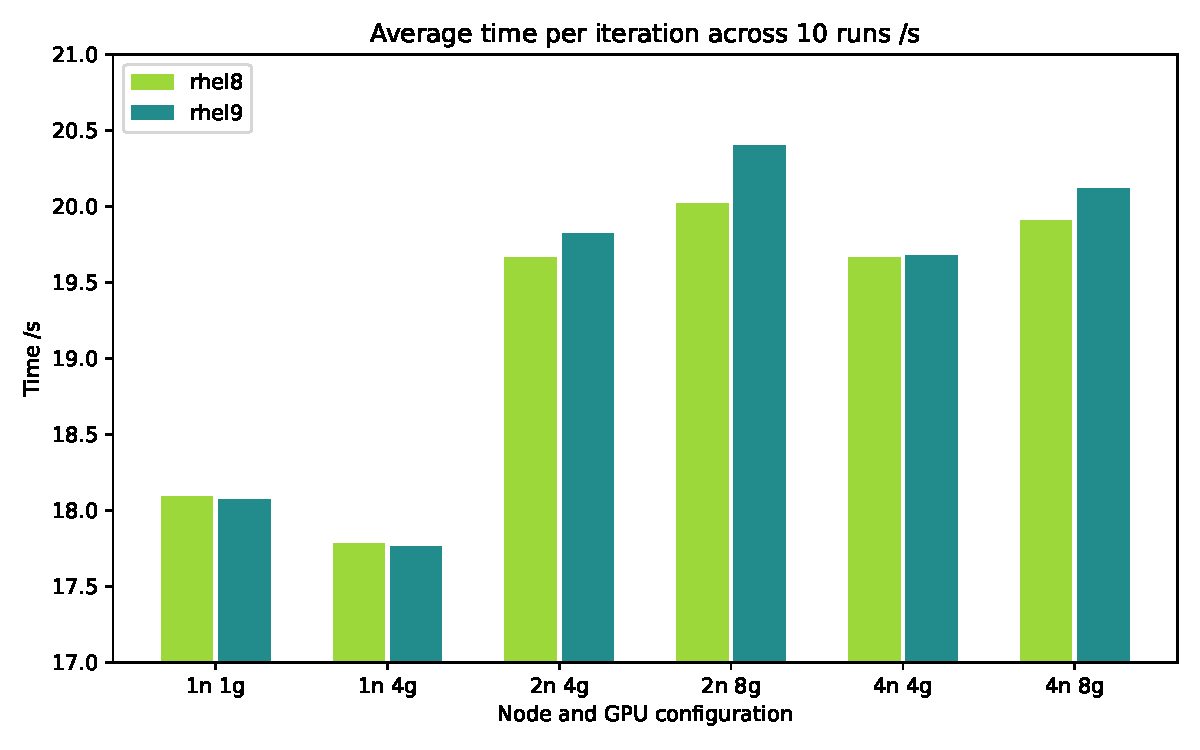
\includegraphics[width=1.0\linewidth]{diagrams/plot-dawn-rhel-comparison.pdf}
\caption{\label{fig:rhel-comparison} Training times for the {\tt rhel8} configuration compared to the {\tt rhel9} configuration. Times shown are for a single iteration averaged across an epoch of 32 samples but with the first iteration skipped. The results are averages across ten runs.}
\end{figure}

These results look similar across the board but not identical. Moreover in some cases we see an increase in speed, in others a decrease. In order to quantify whether the timings for each node and GPU configuration could realistically be considered to have been taken from the same population, we performed a Mann-Whitney U Test \cite{wiki2025mannwhitney}, with the following preconditions:

\begin{enumerate}
    \item The samples are independent.
    \item The data is continuous and ordinal.
\end{enumerate}

Our null hypothesis $H_0$ is that the distributions of the sets of results are identical. Our alternative hypothesis $H_1$ is that the distributions of the sets of results are not identical.

For each configuration of nodes and GPUs we calculate the $U$ statistic as being the smaller of the two values $U_1$ and $U_2$ defined as

$$
U_1 = n_1 n_2 + \frac{n_1 (n_1 + 1)}{2} - \sum_{x \in S_1} \operatorname{rank}(x)
\  \text{ and } \
U_2 = n_1 n_2 + \frac{n_2 (n_2 + 1)}{2} - \sum_{x \in S_2} \operatorname{rank}(x),
$$

where $S_1$ and $S_2$ are the samples taken in each case for {\tt rhel8} and {\tt rhel9} respectively, $n_1 = | S_1 | = 10$, $n_2 = | S_2 | = 10$ and $\operatorname{rank}(x)$ is the position of $x$ when all elements of $S_1$ and $S_2$ are ordered, taking a value between 1 and $n_1 + n_2$ inclusive.

The results for these calculations are detailed in Table \ref{tab:timing-mann-whitney}.

\begin{table}[t]
    \centering
    \begin{tabular}{@{}ll|rr|rrrr@{}}\toprule
      & & \multicolumn{2}{c|}{Average time per step (s)} & & & & \\ 
      Nodes
      & GPUs
      & {\tt rhel8}
      & {\tt rhel9}
      & $U_1$ & $U_2$ & $U$ & Reject $H_0$? \\ \midrule
        1 & 1 & 18.095136 & 18.072201 & 51 & 69 & 51 & No \\
        1 & 4 & 17.780439 & 17.765742 & 61 & 59 & 59 & No \\
        2 & 4 & 19.662787 & 19.823019 & 74 & 46 & 46 & No \\
        2 & 8 & 20.016892 & 20.399696 & 63 & 57 & 57 & No \\
        4 & 4 & 19.664436 & 19.678372 & 61 & 59 & 59 & No \\
        4 & 8 & 19.907159 & 20.116596 & 94 & 26 & 26 & No \\ \bottomrule
    \end{tabular}
    \caption{Mann Whitney U Test calculations comparing the times for runs using the {\tt rhel8} and {\tt rhel9} modules}
    \label{tab:timing-mann-whitney}
\end{table}

Using a two-tailed significance level of 0.05 with these sample sizes the critical value is 23 and, as such, we fail to reject $H_0$ in all cases. This test shows that we are not able to say that the change in modules loaded had an effect on the timings in any of the six cases.

\section{Calculation accuracy}
\label{appendix:calcs}

\subsection{Floating point formats}

We considered error accumulations with matrix operations in Section \ref{section:errors}. Here we delve a little deeper into the details.

Both systems offer a range of different floating point formats: \fpdouble, \fpsingle, \fphalf\ and \bfhalf, amongst others. Each stores a binary representation of a floating point number. Each is comprised of three components: a sign bit (representing positive or negative), a significand and an exponent.

The significand captures the binary digits of the number. The width of this element determines the distance between the largest and smallest digit that can be represented in a single value. This is then binary shifted left or right by the exponent. The size of the exponent determines the range of numbers that the format can represent.

Table \ref{tab:fpwidths} summarises the widths of the sections within each floating point format that we consider.

\begin{table}[t]
    \centering
    \begin{tabular}{@{}lrrrr@{}} \toprule
        Format & Full width & Sign bit width & Significand width & Exponent width \\ \midrule
        \fpdouble & 64 & 1 & 52 & 11 \\
        \fpsingle & 32 & 1 & 23 & 8 \\
        \fphalf & 16 & 1 & 10 & 5 \\
        \bfhalf & 16 & 1 & 7 & 8 \\ \bottomrule
    \end{tabular}
    \caption{Widths of the sections within floating point representations.}
    \label{tab:fpwidths}
\end{table}

These widths are important in the context of these results because they determine the scale of error we'd expect to see in any floating point calculation. In particular, we would expect larger errors to accumulate during addition when the value to be added falls outside the range captured by the significand. Suppose $a, b$ are floating point numbers with $a > b$ and $w_s$ the width of the significand for the format as given in Table \ref{tab:fpwidths}. Then any digits of $b$ that are smaller than $2^{\lfloor \log_2(a) - w_s \rfloor}$ will be lost and therefore increase the error during any addition $a + b$.

\subsection{Matrix generation}

For each experiment we generated random matrices $M$ and $A$ for multiplication and addition respectively. The same seed was used unless stated otherwise, meaning that the same random matrices were generated in each case.

We discovered that generating random numbers on the GPU resulted in different matrices across the two systems. We therefore generated the matrices on the CPU in \fpdouble\ format using \href{https://docs.pytorch.org/docs/stable/generated/torch.rand.html}{\tt torch.rand} and the same seed on both systems. The results were then moved to the GPU before being cast to the appropriate format.

The ranges for the random numbers were selected carefully so that the elementwise values of the result matrices would roughly double every $s = 128$ steps.

We calculated this by setting:
\begin{align*}
a &= \frac{1}{2^{20}} \\
m &= \frac{2^{1 / s}}{n}
\end{align*}

where $n$ is the size of a matrix dimension (either 16 or 1024 in our case) and $s = 128$ is the number of steps before the value doubles.

We then choose the elements of the matrix uniformly at random to fall within the following ranges:
\begin{align*}
a_{i, j} &\in [ a - 0.001, a + 0.001) \\
m_{i, j} &\in [ m - 0.001, m + 0.001)
\end{align*}

The aim is to have the mean values of the $a_{i, j}$ and $m_{i, j}$ be
$a$ and $m$ respectively. We select $a$ to be relatively small
compared to the scale of the elements in the result matrix, in order
that the binary exponent of $a$ falls outside the range of the result
it is to be added to during the addition step. This maximises the opportunity for errors.

Due to the nature of matrix multiplication, if $r_i$ is the average for the elements in the result matrix $R_i$ at step $i$, then $r_{i + 1}$ would take the following approximate value:
$$
r_{i + 1} \approx n m r_i + a
$$

For small enough $a$ and assuming we want our value to double every $s$ steps we can approximate this as:
$$
2 r_i \approx (n m)^s r_i
$$
Rearranging we get:
$$
m \approx \frac{2^{1 / s}}{n}.
$$

In testing we found that this value of $m$ gave good results, roughly doubling the values in the matrix every $s$ steps as intended.

\subsection{Errors in smaller matrices}

In our earlier results we considered matrices with dimension $1024 \times 1024$, but we were also curious to see what would happen with smaller matrices.

The errors for a $16 \times 16$ matrix for the GPUs on Dawn and Baskerville can be seen in Figure \ref{fig:error-comparison-dev-mad-16x16}. As we can see, although lower precision calculations result in larger errors, the errors do not accumulate over time and we see almost identical error performance for both Dawn and Baskerville. This is in stark contrast to the results for the $1024 \times 1024$ matrices. This highlights how errors are cumulative: larger matrices require far more individual calculations during multiplication and addition operations.

\begin{figure}[p]
\centering

\includegraphics[width=1.0\linewidth]{plot-error-dev-mad-16x16.pdf}
\caption{\label{fig:error-comparison-dev-mad-16x16} RMSE for $16 \times 16$ matrix multiply and add operations with various precisions on GPU.}
\end{figure}

\subsection{CPU calculation comparison}

We also considered results from CPU-only calculations for comparison. For the $16 \times 16$ matrices we see the results in Figure \ref{fig:error-comparison-cpu-mad-16x16} and for $1024 \times 1024$ matrices in Figure \ref{fig:error-comparison-cpu-mad-1024x1024-s42}.

As expected we see identical results for the smaller matrices, but we see some small variation in the results for the larger matrices. We show only results for \fpdouble\ and \fpsingle, omitting the half-precision results since these aren't supported on CPU.

The two systems are running different Intel CPUs (Xeon\textsuperscript{\tiny\textregistered} Platinum 8468 and Xeon\textsuperscript{\tiny\textregistered} Platinum 8360Y respectively), but we weren't expecting to see differences. In practice the differences are very small as can be seen in Figure \ref{fig:error-comparison-cpu-mad-1024x1024-s42} and neither appears to give systematically better nor worse results.

\begin{figure}[p]
\centering

\includegraphics[width=1.0\linewidth]{plot-error-cpu-mad-16x16.pdf}
\caption{\label{fig:error-comparison-cpu-mad-16x16} RMSE for $16 \times 16$ matrix multiply and add operations with various precisions on CPU.}
\end{figure}

\begin{figure}[p]
\centering

\includegraphics[width=1.0\linewidth]{plot-error-cpu-mad-1024x1024-s42.pdf}
\caption{\label{fig:error-comparison-cpu-mad-1024x1024-s42} RMSE for $1024 \times 1024$ matrix multiply and add operations with various precisions on CPU.}
\end{figure}

\subsection{Different seeds}

We considered the possibility that the results might not be representative and might be an artifact of the random numbers chosen. To explore this we ran the same calculations with a different seed in order to generate different initial matrices.

We observed an apparently identical error profile, as can be seen in Figure \ref{fig:error-comparison-dev-mad-1024x1024-s43}. The results for CPU were also very similar using this alternative seed, as shown in Figure \ref{fig:error-comparison-cpu-mad-1024x1024-s43}.

\begin{figure}[p]
\centering

\includegraphics[width=1.0\linewidth]{plot-error-dev-mad-1024x1024-s43.pdf}
\caption{\label{fig:error-comparison-dev-mad-1024x1024-s43} RMSE for $1024 \times 1024$ matrix multiply and add operations with different starting matrices on GPU.}
\end{figure}

\begin{figure}[p]
\centering

\includegraphics[width=1.0\linewidth]{plot-error-cpu-mad-1024x1024-s43.pdf}
\caption{\label{fig:error-comparison-cpu-mad-1024x1024-s43} RMSE for $1024 \times 1024$ matrix multiply and add operations with different starting matrices on CPU.}
\end{figure}

\subsection{Multiplication and addition in isolation}

Multiplication and addition are known to have very different error properties for floating point numbers. We were therefore interested to run the same experiments but with just one or other operation in isolation, in case this might shed more light on our previous results.

In Figure \ref{fig:error-comparison-dev-add-1024x1024} we consider the error introduced by repeated matrix addition operations. The results shown in the graph are exactly as we would expect, given the widths of the respective significand and exponent components.

Recall that our addition matrix $A$ was set to have values with a mean of
$$
a = \frac{1}{2^{20}}.
$$

Given this, we'd expect to see significant errors accumulate once $r_i$ has increased beyond $2^{w_s + 1} a$ where $w_s$ is the significand width. For \bfhalf\ with $w_s = 7$ (see Table \ref{tab:fpwidths}) this would be after
$$
\frac{2^8 \frac{1}{2^{20}}}{\frac{1}{2^{20}}} = 2^8 = 256
$$
steps, which we can see very clearly to be the case from the graph. Using the same reasoning, for \fphalf\ format values this would happen after $2^{11} = 2048$ steps and for \fpsingle\ format values after $2^{24} = 16777216$ steps. In both of these latter two cases the graph isn't wide enough for them to appear.

Interestingly it is the case of multiplication that most closely matches our results for the multiply-and-add case. We can see this in Figure \ref{fig:error-comparison-dev-mul-1024x1024}, which shows the errors following repeated multiplications without any addition steps. It appears to be the multiplication step where errors between the two systems are arising.

\begin{figure}[p]
\centering

\includegraphics[width=1.0\linewidth]{plot-error-dev-add-1024x1024.pdf}
\caption{\label{fig:error-comparison-dev-add-1024x1024} RMSE for $1024 \times 1024$ matrix add operations on GPU.}
\end{figure}

\begin{figure}[t]
\centering

\includegraphics[width=1.0\linewidth]{plot-error-dev-mul-1024x1024.pdf}
\caption{\label{fig:error-comparison-dev-mul-1024x1024} RMSE for $1024 \times 1024$ matrix multiply operations on GPU.}
\end{figure}

\subsection{Flat \textit{vs.} Composite}
\label{section:calcflatcomp}

The matrix operations discussed here form the foundations for the more complex calculations of the Aurora model. A natural question is therefore whether we see similar timing differences to those seen when performing fine-tuning of the Aurora model as in Section \ref{section:modelsize}.

To check this we ran four sets of experiments using the same combination of floating point widths as in the earlier sections. For the CPU runs we calculated using \fpdouble and \fpsingle for a total of 128 steps. For the XPU runs we calculated using \fpdouble, \fpsingle, \fphalf and \bfhalf for a total of 256 steps. The times in Table \ref{tab:compflattimings} show the average time across all these formats for a single step.

For the XPU results we ran using both Flat and Composite tiling modes in order to compare the results.

\begin{table}[t]
    \centering
    \begin{tabular}{@{}llr@{}} \toprule
        Device & Tile mode & Average time per step /s \\ \midrule
        CPU & Flat & 0.158091989 \\
        CPU & Composite & 0.155805938 \\
        XPU & Flat & 0.046537613 \\
        XPU & Composite & 0.046697135 \\ \bottomrule
    \end{tabular}
    \caption{Time to run calculations using different configurations.}
    \label{tab:compflattimings}
\end{table}

Apart from the obvious speed up of the XPU over the CPU, the important comparison is between the Composite and Flat results. In this case the timings are very similar with no obvious speed-up using Flat as we saw in Section \ref{section:modelsize} for the full model. The Flat results show a very marginal speed-up of 0.34\%.

This is not especially surprising however, since the data sizes involved with these calculations are very small compared to those for the full model. The data involved fits on a single tile and the timings indicate that the parallelism is also happening on a single tile in both cases.

\subsection{Reproducibility}
\label{section:calcreproducibility}

In Section \ref{section:reproducibility} we saw how on Dawn different runs gave different results unless deterministic execution had been explicitly set.

We were interested to see whether this indeterminism could be seen at the very basic level of matrix operations.

To this end we therefore ran a pair of experiments using the same parameters, performing the matrix operations from the previous sections using the XPU on Dawn. We captured the final outputs of the multiple matrix operations (multiplications and additions) and compared the results from the top left entry of the output matrix.

We were careful to set the same random seed each time, ensuring that the starting point was the same.

Example output captured from the first run using composite tiling can be seen in Table \ref{tab:compresultsfirst}. Each row represents calculations for multiply and addition with fuzzing of matrices of size 1024 and performing 32 steps.

\begin{table}[t]
    \centering
    \begin{tabular}{@{}lll@{}} \toprule
        Precision & CPU & XPU \\ \midrule
        \fpdouble & 0.01825869879179093 & 0.018258698791790956 \\
        \fpsingle & 0.018260332929492966 & 0.01826033927500248 \\
        \fphalf & 0.018260353010952034 & 0.0177001953125 \\
        \bfhalf & 0.01826071641394276 & 0.0390625 \\ \bottomrule
    \end{tabular}
    \caption{Top left entry in the output matrix result using Composite tiling.}
    \label{tab:compresultsfirst}
\end{table}

The results for the two runs when running in composite were
identical. Similarly the results for the two runs when running in flat
were identical. However, in the \fpdouble\ case, the output from the
XPU when running in Composite mode was very marginally different from
the output when running in Flat mode, as can be seen in Table
\ref{tab:flatresultsfirst}. It is not clear why this might be happening, but we note this is not an example of non-deterministic output, but rather differences due to different configurations.

\begin{table}[t]
    \centering
    \begin{tabular}{@{}lll@{}} \toprule
        Precision & CPU & XPU \\ \midrule
        \fpdouble & 0.01825869879179093 & 0.01825869879179094 \\
        \fpsingle & 0.018260332929492966 & 0.01826033927500248 \\
        \fphalf & 0.018260353010952034 & 0.0177001953125 \\
        \bfhalf & 0.01826071641394276 & 0.0390625 \\ \bottomrule
    \end{tabular}
    \caption{Top left entry in the output matrix result using Flat tiling.}
    \label{tab:flatresultsfirst}
\end{table}

These results tell us that the non-deterministic nature of the model was likely caused by higher level issues with the Torch code (\textit{e.g.,} tensors being used uninitialised) rather than differences at the level of basic maths operations.

\subsection{Comparison with Aurora}
\label{section:calccomparisonaurora}

A natural question that arises is whether the calculation accuracies seen here are commensurate with those seen when performing inference from Aurora.

The objective with the tests here was to break the task down into its most simple components. Unfortunately this leaves a large gulf between the matrix and add operations tested and the calculations being performed for even the simplest of operations with Aurora.

At this point in time we don't have a good method for comparing these results with the errors seen with Aurora.
